\documentclass[12pt]{article}
\usepackage[ukrainian,english]{babel}
\usepackage[utf8]{inputenc}
\usepackage[T2A]{fontenc} 

\usepackage{sbc-template}

\usepackage{graphicx,url}



 
% UTF-8 encoding is recommended by ShareLaTex
\usepackage{verbatim}
\usepackage{listings}
\usepackage{xcolor}



\definecolor{verde}{rgb}{0,0.5,0}


\begin{document} 

\section{\MakeUppercase{Система управління базою даних }}


Система управління базою даних (СУБД) - найважливіший компонент
інформаційної системи. Для створення і управління інформаційною
системою СУБД необхідна в тій же мірі, як для розробки програми на
алгоритмічній мові необхідний транслятор. Основні функції СУБД:
 управління даними в зовнішній пам'яті (на дисках);
 управління даними в оперативній пам'яті; журналізація змін і
відновлення бази даних після збоїв;

\section{Referencial Teórico} \label{sec:firstpage}

C?????? ?????????? ????? ????? (????) - ????????????? ?????????
????????????? ???????. ??? ????????? ? ?????????? ?????????????
???????? ???? ????????? ? ??? ?? ????, ?? ??? ???????? ???????? ??
????????????? ???? ?????????? ??????????. ??????? ??????? ????:
? ?????????? ?????? ? ????????? ???'??? (?? ??????);
? ?????????? ?????? ? ??????????? ???'???; ???????????? ???? ?
??????????? ???? ????? ????? ?????;

\subsection{Sobre o Referencial teórico}
Referencial teórico é a fundamentação do estudo/pesquisa. Os assuntos teóricos explorados pelos alunos nesta seção devem ter relação direta com o tema da pesquisa e estar alinhados aos objetivos traçados.

Nesta seção, o aluno pode abordar também os estudos relacionados ao tema. É importante o uso de artigos publicados em anais e periódicos recentes.


\section{Metodologia}

Descreve os métodos e técnicas utilizados na pesquisa

\subsection{Sobre seções e parágrafos}

Os títulos das seções devem estar em negrito, fonte 13pt, alinhados a esquerda. A linha do título da seção deve possuir 12pts de espaçamento antes do seu início. A numeração das seções é opcional, embora recomendado. O primeiro parágrafo de cada seção não deve ser tabulado, enquanto que as primeiras linhas dos parágrafos subsequentes devem ser tabulados em 1.27 cm.

Os títulos das subseções devem estar em negrito, 12pt, alinhados a esquerda.


\section{Análise dos dados}\label{sec:analisedosdados}

Nesta seção, o aluno descreve o efetivo procedimento metodológico adotado e aponta os resultados da pesquisa. Na análise de dados, é  aconselhável o uso de tabelas, figuras, linhas de códigos etc para representar os resultados do estudo.

As Tabelas, Quadros e Figuras, assim como as legendas de Tabelas, Quadros e Figuras devem estar centralizadas se conterem apenas em uma linha (Figura~\ref{fig:figura1}), caso contrário devem estar tabuladas em 0.8cm em ambas as margens, como mostra a Figura~\ref{fig:figura2}. 

\begin{figure}[ht]
\centering
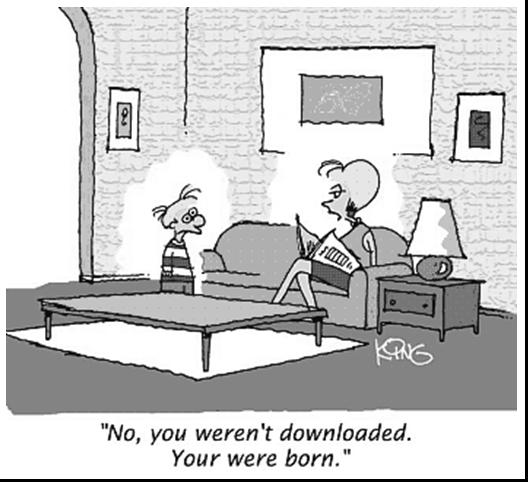
\includegraphics[width=.3\textwidth]{fig1.jpg}
\caption{Exemplo de figura}
\label{fig:figura1}
\end{figure}

As legendas devem ser escritas na fonte “Helvetica”, Tamanho 10pts, negrito, com espaço de 6pts antes e depois de cada legenda. Sempre que possível, procure colocar a figura delimitada por um quadro (Figura~\ref{fig:figura1} e Figura~\ref{fig:figura2})

\begin{figure}[!ht]
\centering
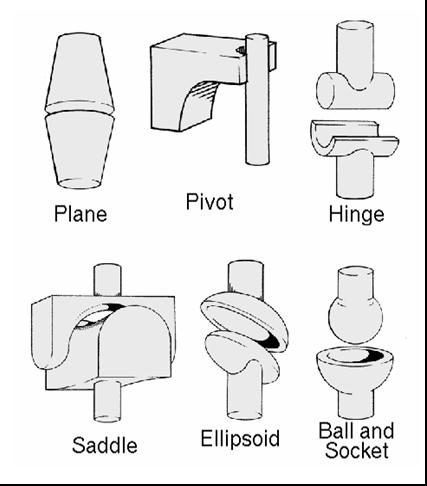
\includegraphics[width=.2\textwidth]{fig2.jpg}
\caption{Essa figura foi referenciada na Seção~\ref{sec:analisedosdados}.}
\caption{Fonte: SBC.}
\label{fig:figura2}
\end{figure}

Em tabelas, tente evitar o uso de fundos coloridos ou preenchidos, assim como linhas duplas na borda, ou linhas desnecessárias. Quando \cite{knuth:84} relatar dados empíricos, não faça uso de mais dígitos decimais do que o necessário. A legenda da tabela deve ser colocada antes da tabela (veja Tabela 1) e a fonte usada na legenda deve ser Helvetica, tamanho 10pts, negrito, com 6pts de espaço antes e depois de cada legenda.

\begin{table}[!ht]
\centering
\caption{Exemplo de tabela de 3 colunas e 2 linhas}
\label{tab:exTable1}
\smallskip
\begin{tabular}{l c c}
\hline
& Value 1 & Value 2\\[0.5ex]
\hline
&&\\[-2ex]
Case 1 & 1.0 $\pm$ 0.1 & 1.75$\times$10$^{-5}$ $\pm$ 5$\times$10$^{-7}$\\[0.5ex]
\hline
&&\\[-2ex]
Case 2 & 0.003(1) & 100.0\\[0.5ex]
\hline
\end{tabular}
\end{table}

\subsection{Código fonte}
A inserção de código fonte deve ser por meio

\begin{lstlisting}

int main(){
  int a,b,c;
  float x;
  printf("informe o tamanho do lado do quadrado");
  scanf("%d", &a);
  printf("A area do quadrado %d", b=area(a));
  printf("Duas vezes o valor do lado do quadrado %d", c=aumenta(a));

\end{lstlisting}



\section{Considerações Finais}

Referências bibliográficas devem ser utilizadas dentro de um estilo uniforme e não ambíguo. A SBC sugere os seguintes formatos para referências: \cite{knuth:84}, \cite{boulic:91}, e \cite{smith:99}.

\bibliographystyle{sbc}
\bibliography{sbc-template}

\end{document}
